\documentclass{standalone}
\usepackage{tikz} 
\usepackage{epsf,graphicx,subfig}
\usepackage{color}
\usepackage{amssymb,amsmath}
\usepackage{scalefnt}
\usetikzlibrary{positioning}
%include other needed packages here   
\begin{document}

\begin{tikzpicture}

\definecolor{lungColor}{rgb}{0.2353, 0.6078, 0.8235}
\definecolor{chestWallColor}{rgb}{0.5294, 0.7843, 0.6078}
\definecolor{ribColor}{rgb}{0.0000, 0.4510, 0.1961}
\definecolor{pectoralColor}{rgb}{0.6510, 0.3490, 1.0000}
\definecolor{fibroGlandColor}{rgb}{1.0000, 1.0000, 0.0000}
\definecolor{fatColor}{rgb}{0.9804, 0.5882, 0.1176}
\definecolor{skinColor}{rgb}{0.9804, 0.7255, 0.7451}
\definecolor{unkTissueColor}{rgb}{0.6000, 0.3020, 0.2510}
\definecolor{bgColor}{rgb}{0.0000, 0.0000, 0.0000}
\definecolor{lesionColor}{rgb}{1.0000, 0.2510, 0.0000}
\definecolor{boundaryColor}{rgb}{0.8784, 0.8784, 0.7529}

\tikzset{labelSt/.style=
{anchor=north west,rectangle,
node distance=1.71pt,
scale=.6,
minimum width=1pt,minimum height=1pt,
}}

\node[anchor=south west,inner sep=0] (imgNode) at (0,0) {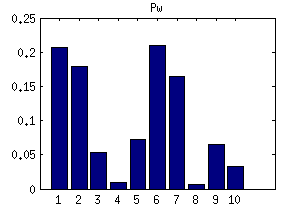
\includegraphics[trim = 5 5 18 0, clip,width=2.93cm,]{classPrior}};

\draw[] (imgNode.south west) +(14pt,3.5pt) node[labelSt, draw=bgColor, fill=bgColor] (bgName) {} ;
\draw[] node[labelSt,draw=lungColor, fill=lungColor,right=of bgName] (lungName) {};
\draw[] node[labelSt, draw=chestWallColor,right=of lungName, fill=chestWallColor] (cwName) {} ;
\draw[] node[labelSt, draw=ribColor, fill=ribColor,right=of cwName] (ribName) {} ;
\draw[] node[labelSt, draw=pectoralColor, fill=pectoralColor,right=of ribName] (pectoralName) {} ;
\draw[] node[labelSt, draw=fibroGlandColor, fill=fibroGlandColor,right=of pectoralName] (fibroGlandName) {} ;
\draw[] node[labelSt, draw=fatColor, fill=fatColor,right=of fibroGlandName] (fatName) {} ;
\draw[] node[labelSt, draw=skinColor, fill=skinColor,right=of fatName] (skinName) {} ;
\draw[] node[labelSt, draw=lesionColor, fill=lesionColor,right=of skinName] (lesionName) {} ;
\draw[] node[labelSt, draw=boundaryColor, fill=boundaryColor,right=of lesionName] (boundaryName) {} ;

\end{tikzpicture}

\end{document}